  \usetikzlibrary {backgrounds,fit}
    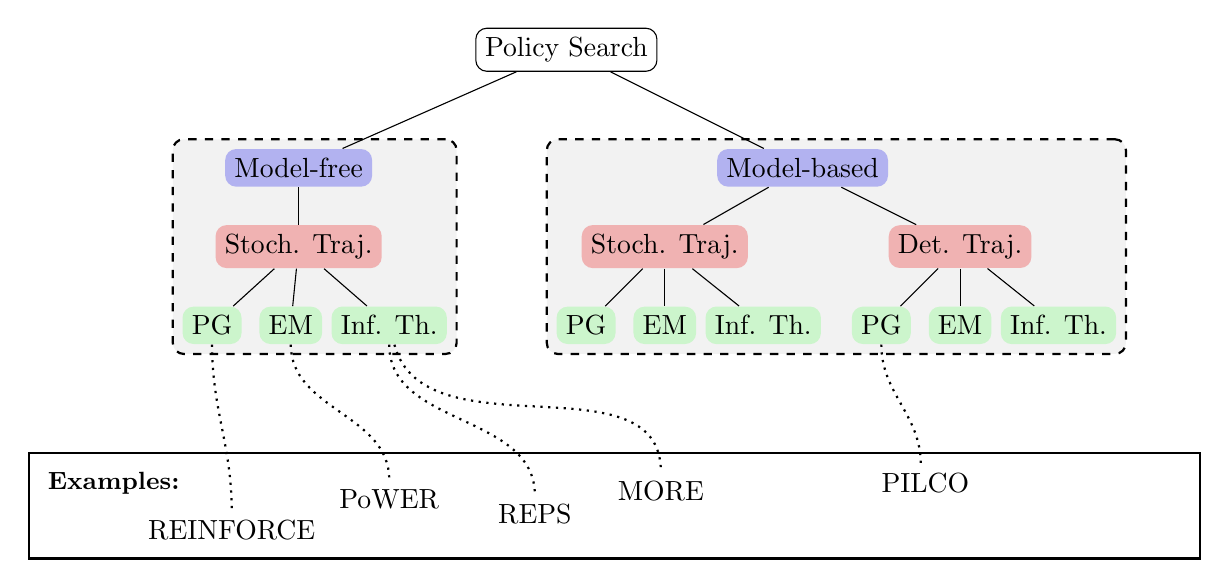
\begin{tikzpicture}
      \draw (1, 0.5) node [draw=black, rounded corners] (data) {Policy Search};

      \draw (-2.4, -1) node [fill=blue!80!black!30, rounded corners](model_free) {Model-free};
      \draw [-] (data) -- (model_free);      
      \draw (-2.4, -2) node [fill=red!80!black!30, rounded corners](free) {Stoch. Traj.};
      \draw [-] (model_free) -- (free);      
      \draw (-3.5, -3) node [fill=green!80!black!20, rounded corners](free_pg) {PG};
      \draw (-2.5, -3) node [fill=green!80!black!20, rounded corners](free_em) {EM};
      \draw (-1.25, -3) node [fill=green!80!black!20, rounded corners](free_inf) {Inf. Th.};
      \draw [-] (free) -- (free_pg);
      \draw [-] (free) -- (free_em);
      \draw [-] (free) -- (free_inf);
      
      
      \draw (4, -1) node [fill=blue!80!black!30, rounded corners] (model) {Model-based};
      \draw [-] (data) -- (model);
      
      \draw (2.25, -2) node [fill=red!80!black!30, rounded corners] (model_stoch) {Stoch. Traj.};
      \draw [-] (model) -- (model_stoch);      
      \draw (1.25, -3) node [fill=green!80!black!20, rounded corners](stoch_pg) {PG};
      \draw (2.25, -3) node [fill=green!80!black!20, rounded corners](stoch_em) {EM};
      \draw (3.5, -3) node [fill=green!80!black!20, rounded corners](stoch_inf) {Inf. Th.};
      \draw [-] (model_stoch) -- (stoch_pg);
      \draw [-] (model_stoch) -- (stoch_em);
      \draw [-] (model_stoch) -- (stoch_inf);

      
      \draw (6, -2) node [fill=red!80!black!30, rounded corners] (model_det) {Det. Traj.};
      \draw [-] (model) -- (model_det);      
      \draw (5, -3) node [fill=green!80!black!20, rounded corners](det_pg) {PG};
      \draw (6, -3) node [fill=green!80!black!20, rounded corners](det_em) {EM};
      \draw (7.25, -3) node [fill=green!80!black!20, rounded corners](det_inf) {Inf. Th.};
      \draw [-] (model_det) -- (det_pg);
      \draw [-] (model_det) -- (det_em);
      \draw [-] (model_det) -- (det_inf);

      %%%%%%%%%%%%%%%%%%%%%%%%%%%%%%%%%%%%%%%%%%%%%%%%%%%%%%%%%%%%%%
      % Examples
      %%%%%%%%%%%%%%%%%%%%%%%%%%%%%%%%%%%%%%%%%%%%%%%%%%%%%%%%%%%%%%
      \draw (-4.75, -5) node (examples) {\small \textbf{Examples:}};      
      \draw (-3.25, -5.6) node (reinforce) {REINFORCE};
      \draw (-1.25, -5.2) node (power) {PoWER};
      \draw (0.6, -5.4) node (reps) {REPS};
      \draw (2.2, -5.1) node (more) {MORE};      
      \draw [thick, dotted] (free_pg) to[out=-90,in=90] (reinforce);
      \draw [thick, dotted] (free_em) to[out=-90,in=90] (power);
      \draw [thick, dotted] (free_inf) to[out=-90,in=90] (reps);
      \draw [thick, dotted] (free_inf) to[out=-75,in=90] (more);      

      
      % \draw (4, -5.75) node (pegasus) {PEGASUS};
      \draw (5.5, -5) node (pilco)
      {$~~~~~~~~\quad\quad\quad\quad\quad$ PILCO $~~~~~~~\quad\quad\quad\quad\quad$};
      \draw [thick, dotted] (det_pg) to[out=-90,in=90] (pilco);

      \begin{scope}[on background layer]
        \node [thick, dashed, draw=black, rounded corners, fill=black!5,fit=
        (model_free) (free) (free_pg) (free_em) (free_inf)]{};
      \end{scope}
      
      \begin{scope}[on background layer]
        \node [thick, dashed, draw=black, rounded corners, fill=black!5,fit=
        (model) (model_det) (model_stoch)
        (det_pg) (det_em) (det_inf)
        (stoch_pg) (stoch_em) (stoch_inf)]{};
      \end{scope}
      
      \begin{scope}[on background layer]
        \node [thick, draw=black,fit=
        (examples)
        (reinforce) (power)
        (reps) (pilco)]{};
      \end{scope}
    \end{tikzpicture}
